\section{Protocolo Experimental}
\label{sec:protocolo_experimental}

Para comparar Sockets TCP y gRPC en igualdad de condiciones y evitar conclusiones basadas en una única ejecución aislada, el equipo implementó un protocolo automatizado en \texttt{src/run\_experiments.py} que ejecuta ambos mecanismos de forma consecutiva sobre la misma máquina, con los mismos puertos (\texttt{5000}, \texttt{5001} y \texttt{5002}) y la misma carga útil.

\subsection{Entorno de ejecución y condiciones de la máquina}

Las corridas definitivas fueron registradas automáticamente en \texttt{data/machine\_info.json} mediante \texttt{src/common/machine\_info.py} antes de iniciar las mediciones. La Tabla~\ref{tab:hardware_entorno} resume el entorno físico y de software controlado durante todo el experimento.

\begin{table}[htbp]
\centering
\caption{Condiciones de hardware y software registradas en \texttt{data/machine\_info.json}.}
\label{tab:hardware_entorno}
\small
\begin{tabular}{lp{10.2cm}}
\toprule
Parámetro & Valor registrado en el entorno de pruebas \\
\midrule
Equipo (\emph{hostname}) & \texttt{DESKTOP-OSLA9DF} \\
Sistema operativo & Windows 11 (\texttt{10.0.26200}, arquitectura AMD64) \\
Procesador & AMD Ryzen 5 7535HS with Radeon Graphics (12 hilos lógicos) \\
Memoria RAM total & 15,32\,GB \\
Intérprete de Python & CPython 3.12.10 (entorno virtual \texttt{.venv}) \\
Dependencias exactas & \texttt{grpcio==1.85.3}, \texttt{protobuf==7.36.2}, \texttt{pandas==3.0.2}, \texttt{matplotlib==3.11.2}, \texttt{numpy==2.4.4} \\
Modo de despliegue & Tres procesos locales independientes en \texttt{127.0.0.1} (\texttt{nodo-A}, \texttt{nodo-B}, \texttt{nodo-C}) \\
Fecha de captura (local) & 19 de noviembre de 2026, 21:32:53\,UTC$-5$ \\
\bottomrule
\end{tabular}
\end{table}

\subsection{Diseño de corridas, tamaños de mensaje e integridad de datos}

Cada mecanismo sigue exactamente la misma secuencia experimental:
\begin{enumerate}
  \item \textbf{Arranque aislado de los tres procesos:} \texttt{run\_experiments.py} inicia \texttt{nodo-A:5000}, \texttt{nodo-B:5001} y \texttt{nodo-C:5002} con el servidor del mecanismo bajo prueba, espera a que los tres puertos acepten conexiones y, al terminar, finaliza los procesos y verifica la liberación de puertos antes de lanzar el segundo mecanismo.
  \item \textbf{Intercambios con reloj de Lamport:} se ejecutan 20 intercambios predefinidos compartidos entre \texttt{client.py} y \texttt{client\_grpc.py} (\texttt{EXCHANGE\_STEPS}), incluyendo dos pares de envíos simultáneos sincronizados mediante barrera (\texttt{ex-01}/\texttt{ex-02} y \texttt{ex-09}/\texttt{ex-10}). Cada envío y recepción se persiste en formato CSV y JSON dentro de \texttt{/data/} (40 eventos por mecanismo).
  \item \textbf{Calentamiento y repeticiones válidas:} para cada tamaño de carga útil ---mensaje corto de 100\,B (\texttt{100B}) y mensaje largo de 10\,240\,B (\texttt{10KB})--- se ejecuta primero una corrida de calentamiento de 100 envíos (\texttt{run\_id=0}, con \texttt{is\_warmup=True}) que el análisis descarta, seguida de cinco repeticiones válidas de 100 envíos (\texttt{run\_id=1..5}).
  \item \textbf{Modo secuencial y modo concurrente:} en modo secuencial, \texttt{nodo-A} transmite en \emph{round-robin} hacia \texttt{nodo-B} y \texttt{nodo-C} (500 muestras válidas por tamaño). En modo concurrente, los tres clientes se sincronizan con una barrera de tres hilos (\texttt{threading.Barrier}) y envían 100 mensajes cada uno por repetición (1\,500 muestras válidas por tamaño). En gRPC se activó un \emph{subchannel pool} local por cliente para usar conexiones HTTP/2 independientes, igualando el aislamiento de TCP.
  \item \textbf{Medición e integridad:} el tiempo de ida y vuelta (RTT) se mide con \texttt{time.perf\_counter()} sobre conexiones ya establecidas. En total se registraron 4\,800 filas por mecanismo (4\,000 válidas y 800 de calentamiento), protegidas con sus sumas de verificación en \texttt{data/SHA256SUMS} para comprobar que no se alteraron después.
\end{enumerate}

\section{Resultados Experimentales}
\label{sec:resultados}

Las tablas y gráficos de esta sección se generaron automáticamente a partir de los archivos crudos \texttt{data/latency\_sockets.csv} y \texttt{data/latency\_grpc.csv} mediante \texttt{python -m analysis.run\_analysis}, descartando las 1\,600 muestras de calentamiento y procesando las 8\,000 mediciones válidas restantes.

\begin{table}[htbp]
\centering
\caption{Latencia RTT y rendimiento por mecanismo y tamaño -- modo secuencial}
\label{tab:latencias_sequential}
\small
\begin{tabular}{llrrrrrr}
\toprule
Mecanismo & Tamano & $n$ & Media (ms) & Mediana (ms) & Desv. Est. (ms) & P95 (ms) & Rend. (msg/s) \\
\midrule
gRPC & 100B & 500 & 0.4655 & 0.4398 & 0.0928 & 0.6317 & 2133.2 \\
gRPC & 10KB & 500 & 0.6757 & 0.6445 & 0.1607 & 0.9781 & 1464.1 \\
Sockets TCP & 100B & 500 & 0.0884 & 0.0779 & 0.0221 & 0.1315 & 10860.9 \\
Sockets TCP & 10KB & 500 & 0.1410 & 0.1348 & 0.0317 & 0.2061 & 6895.5 \\
\bottomrule
\end{tabular}
\end{table}

\begin{table}[htbp]
\centering
\caption{Latencia RTT y rendimiento por mecanismo y tamaño -- modo concurrente (3 clientes)}
\label{tab:latencias_concurrent}
\small
\begin{tabular}{llrrrrrr}
\toprule
Mecanismo & Tamano & $n$ & Media (ms) & Mediana (ms) & Desv. Est. (ms) & P95 (ms) & Rend. (msg/s) \\
\midrule
gRPC & 100B & 1500 & 0.6007 & 0.5187 & 0.2951 & 0.9789 & 5153.6 \\
gRPC & 10KB & 1500 & 0.5774 & 0.5285 & 0.1592 & 0.8823 & 5151.1 \\
Sockets TCP & 100B & 1500 & 0.1329 & 0.1192 & 0.0600 & 0.2043 & 21449.7 \\
Sockets TCP & 10KB & 1500 & 0.1988 & 0.1836 & 0.0570 & 0.3043 & 14577.6 \\
\bottomrule
\end{tabular}
\end{table}

\begin{table}[htbp]
\centering
\caption{Variación porcentual de gRPC respecto a Sockets TCP (valores positivos favorecen a gRPC)}
\label{tab:comparacion_relativa}
\footnotesize
\begin{tabular}{llrrrrr}
\toprule
Modo & Tamaño & TCP media (ms) & gRPC media (ms) & $\Delta$ media (\%) & $\Delta$ P95 (\%) & $\Delta$ rend. (\%) \\
\midrule
Concurrente (3 clientes) & 100B & 0.1329 & 0.6007 & -352.15 & -379.12 & -75.97 \\
Concurrente (3 clientes) & 10KB & 0.1988 & 0.5774 & -190.39 & -189.95 & -64.66 \\
Secuencial & 100B & 0.0884 & 0.4655 & -426.77 & -380.49 & -80.36 \\
Secuencial & 10KB & 0.1410 & 0.6757 & -379.12 & -374.56 & -78.77 \\
\bottomrule
\end{tabular}
\end{table}


En modo secuencial (Tabla~\ref{tab:latencias_sequential}), Sockets TCP obtuvo una latencia media de 0,0884\,ms (P95 de 0,1315\,ms) con 100\,B y de 0,1410\,ms (P95 de 0,2061\,ms) con 10\,KB, alcanzando rendimientos de 10\,860,9 y 6\,895,5\,msg/s respectivamente. Bajo las mismas condiciones, gRPC registró una media de 0,4655\,ms (P95 de 0,6317\,ms) en 100\,B y de 0,6757\,ms (P95 de 0,9781\,ms) en 10\,KB, con rendimientos de 2\,133,2 y 1\,464,1\,msg/s.

En modo concurrente con tres clientes simultáneos (Tabla~\ref{tab:latencias_concurrent}), el rendimiento agregado creció en ambos mecanismos: Sockets TCP alcanzó 21\,449,7\,msg/s en 100\,B (latencia media de 0,1329\,ms, 1,97$\times$ el rendimiento secuencial) y 14\,577,6\,msg/s en 10\,KB (0,1988\,ms, 2,11$\times$). Por su parte, gRPC escaló proporcionalmente más al pasar a tres hilos: alcanzó 5\,153,6\,msg/s en 100\,B (2,42$\times$ frente a secuencial) y 5\,151,1\,msg/s en 10\,KB (3,52$\times$ frente a secuencial), manteniendo prácticamente constante su rendimiento entre 100\,B y 10\,KB (variación de apenas $-$0,05\,\%) e incluso reduciendo su media de 0,6007\,ms a 0,5774\,ms y su P95 de 0,9789\,ms a 0,8823\,ms. La Tabla~\ref{tab:comparacion_relativa} sintetiza las diferencias porcentuales exactas en los cuatro escenarios.

\begin{figure}[htbp]
\centering
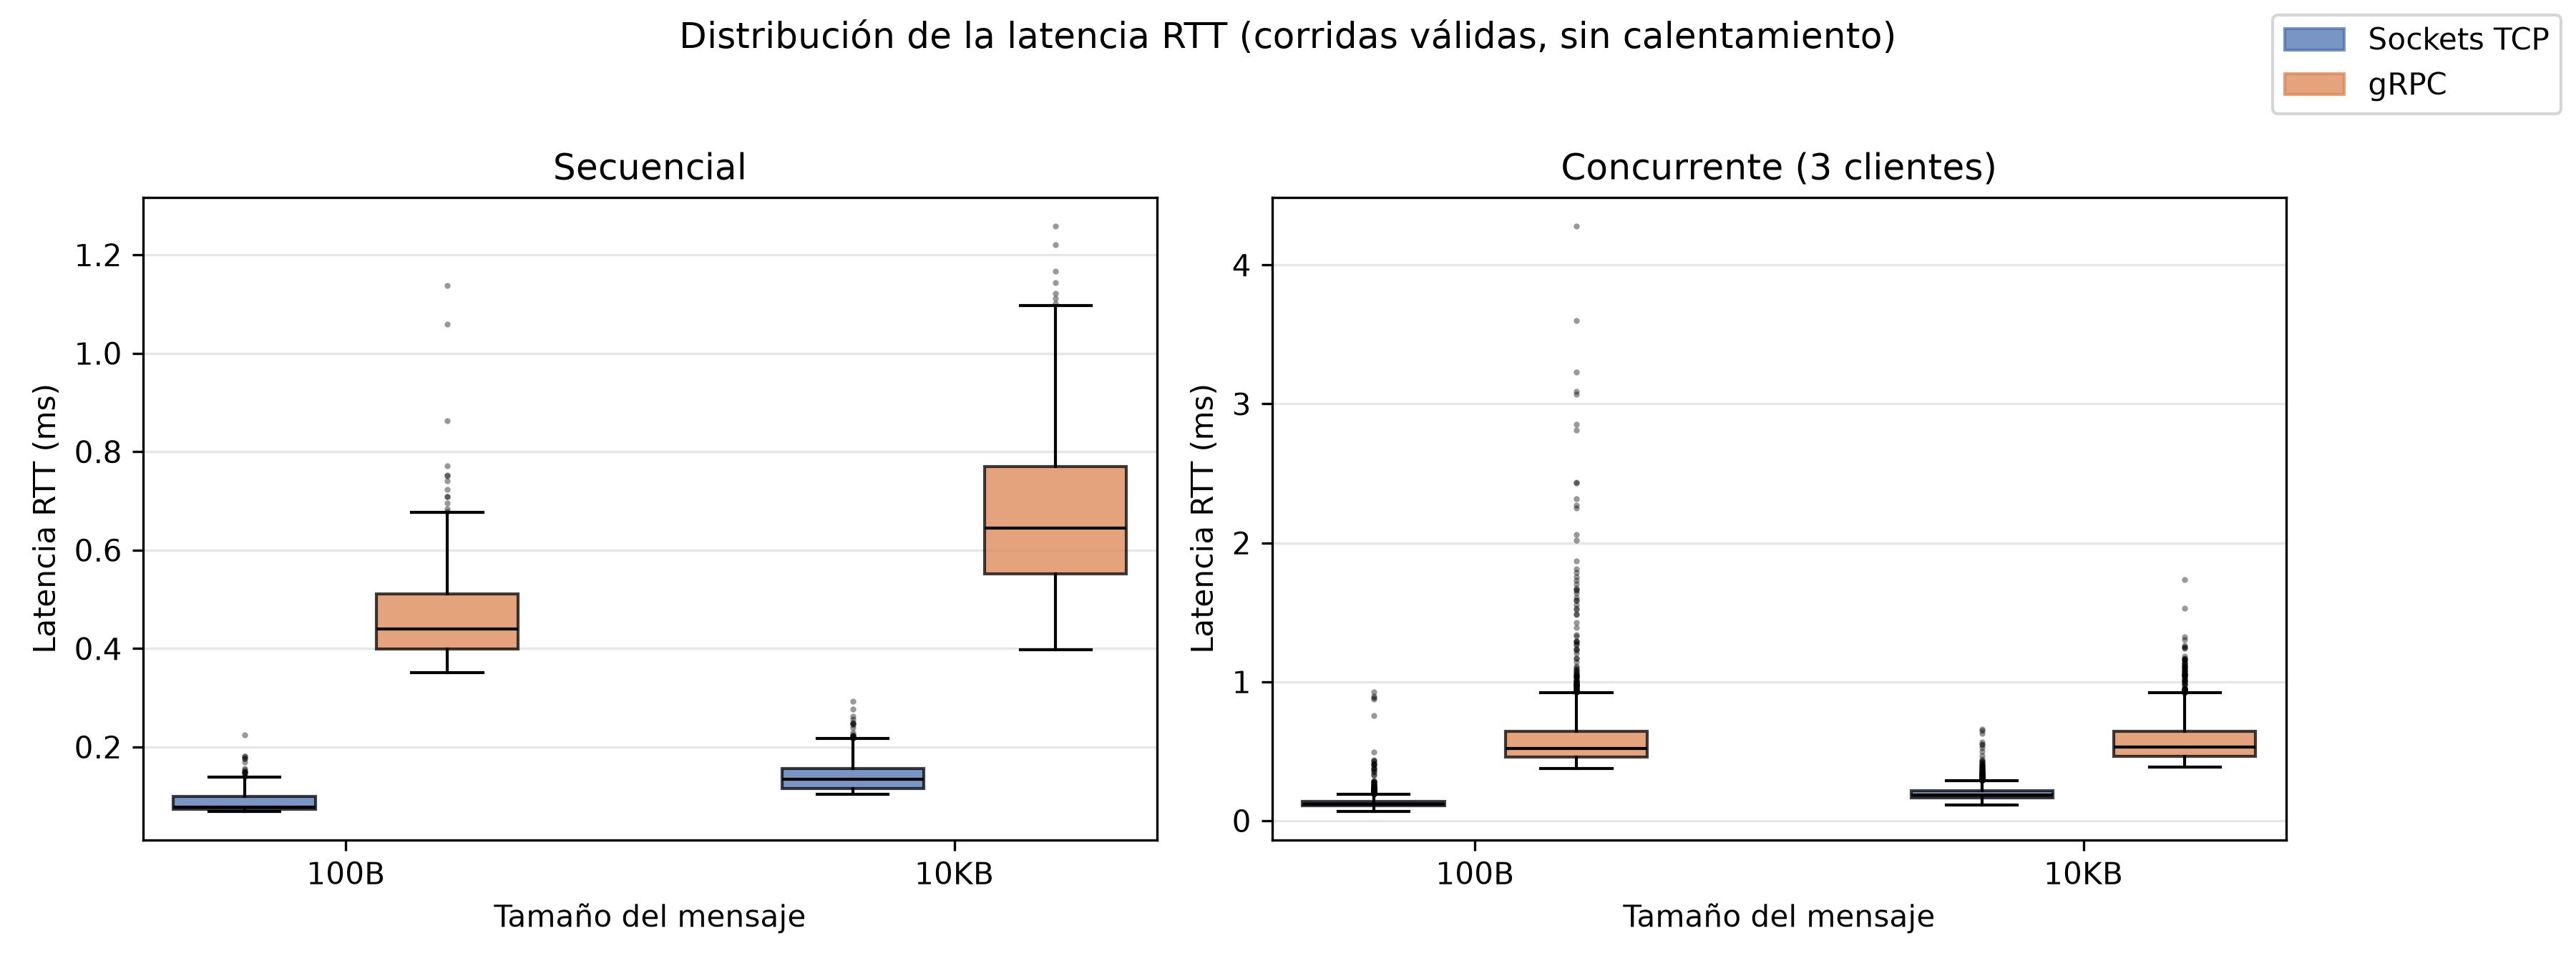
\includegraphics[width=0.96\textwidth]{figures/boxplot_latencias.png}
\caption{Distribución de latencias RTT (diagrama de cajas) para Sockets TCP y gRPC en modos secuencial y concurrente, excluyendo corridas de calentamiento (300\,DPI).}
\label{fig:boxplot_latencias}
\end{figure}

\begin{figure}[htbp]
\centering
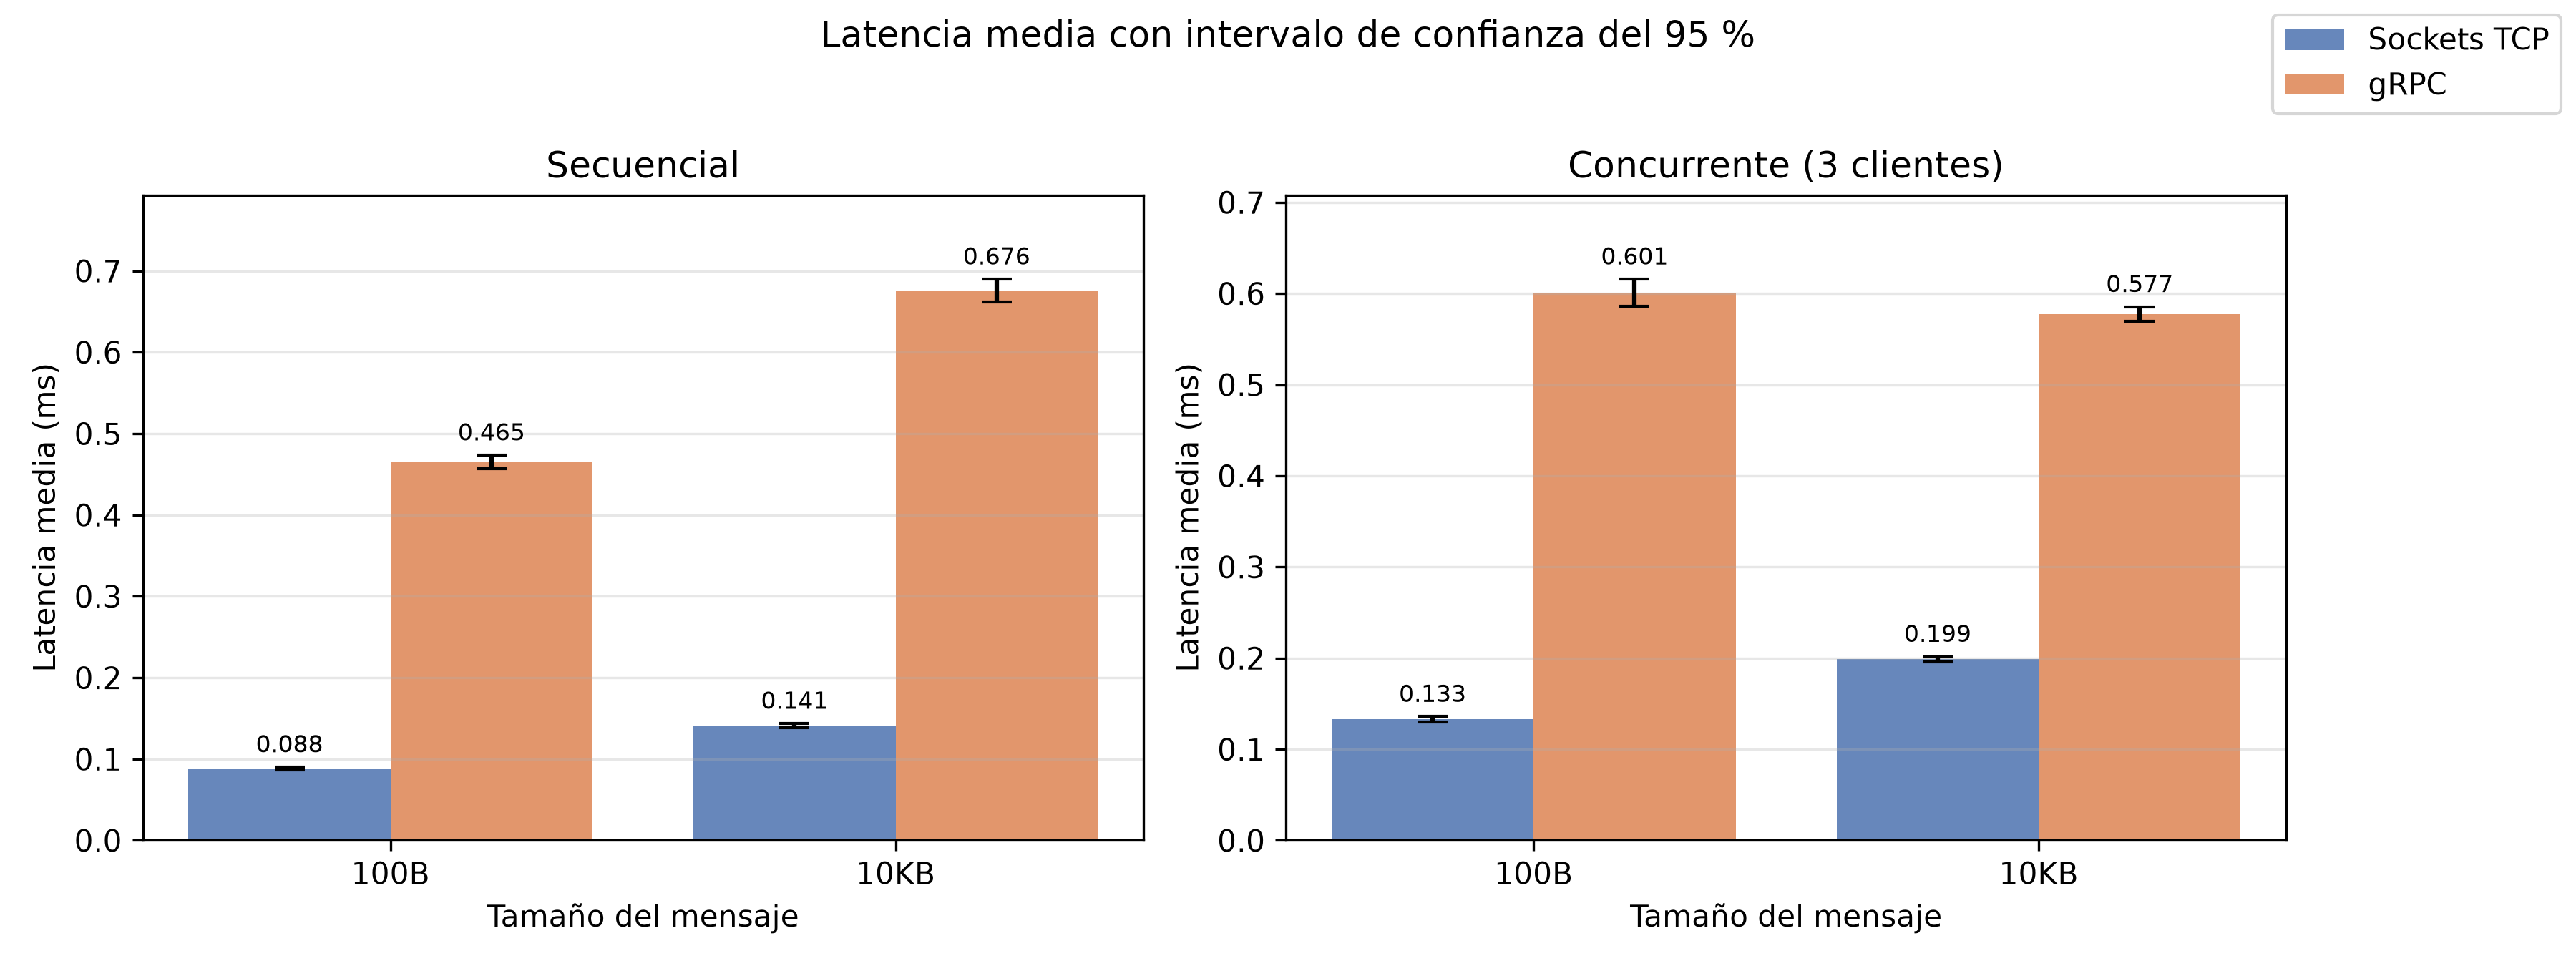
\includegraphics[width=0.96\textwidth]{figures/barras_latencia_ic95.png}
\caption{Latencia media RTT con intervalos de confianza del 95\,\% para ambos mecanismos y tamaños de mensaje (300\,DPI).}
\label{fig:barras_latencia_ic95}
\end{figure}

\begin{figure}[htbp]
\centering
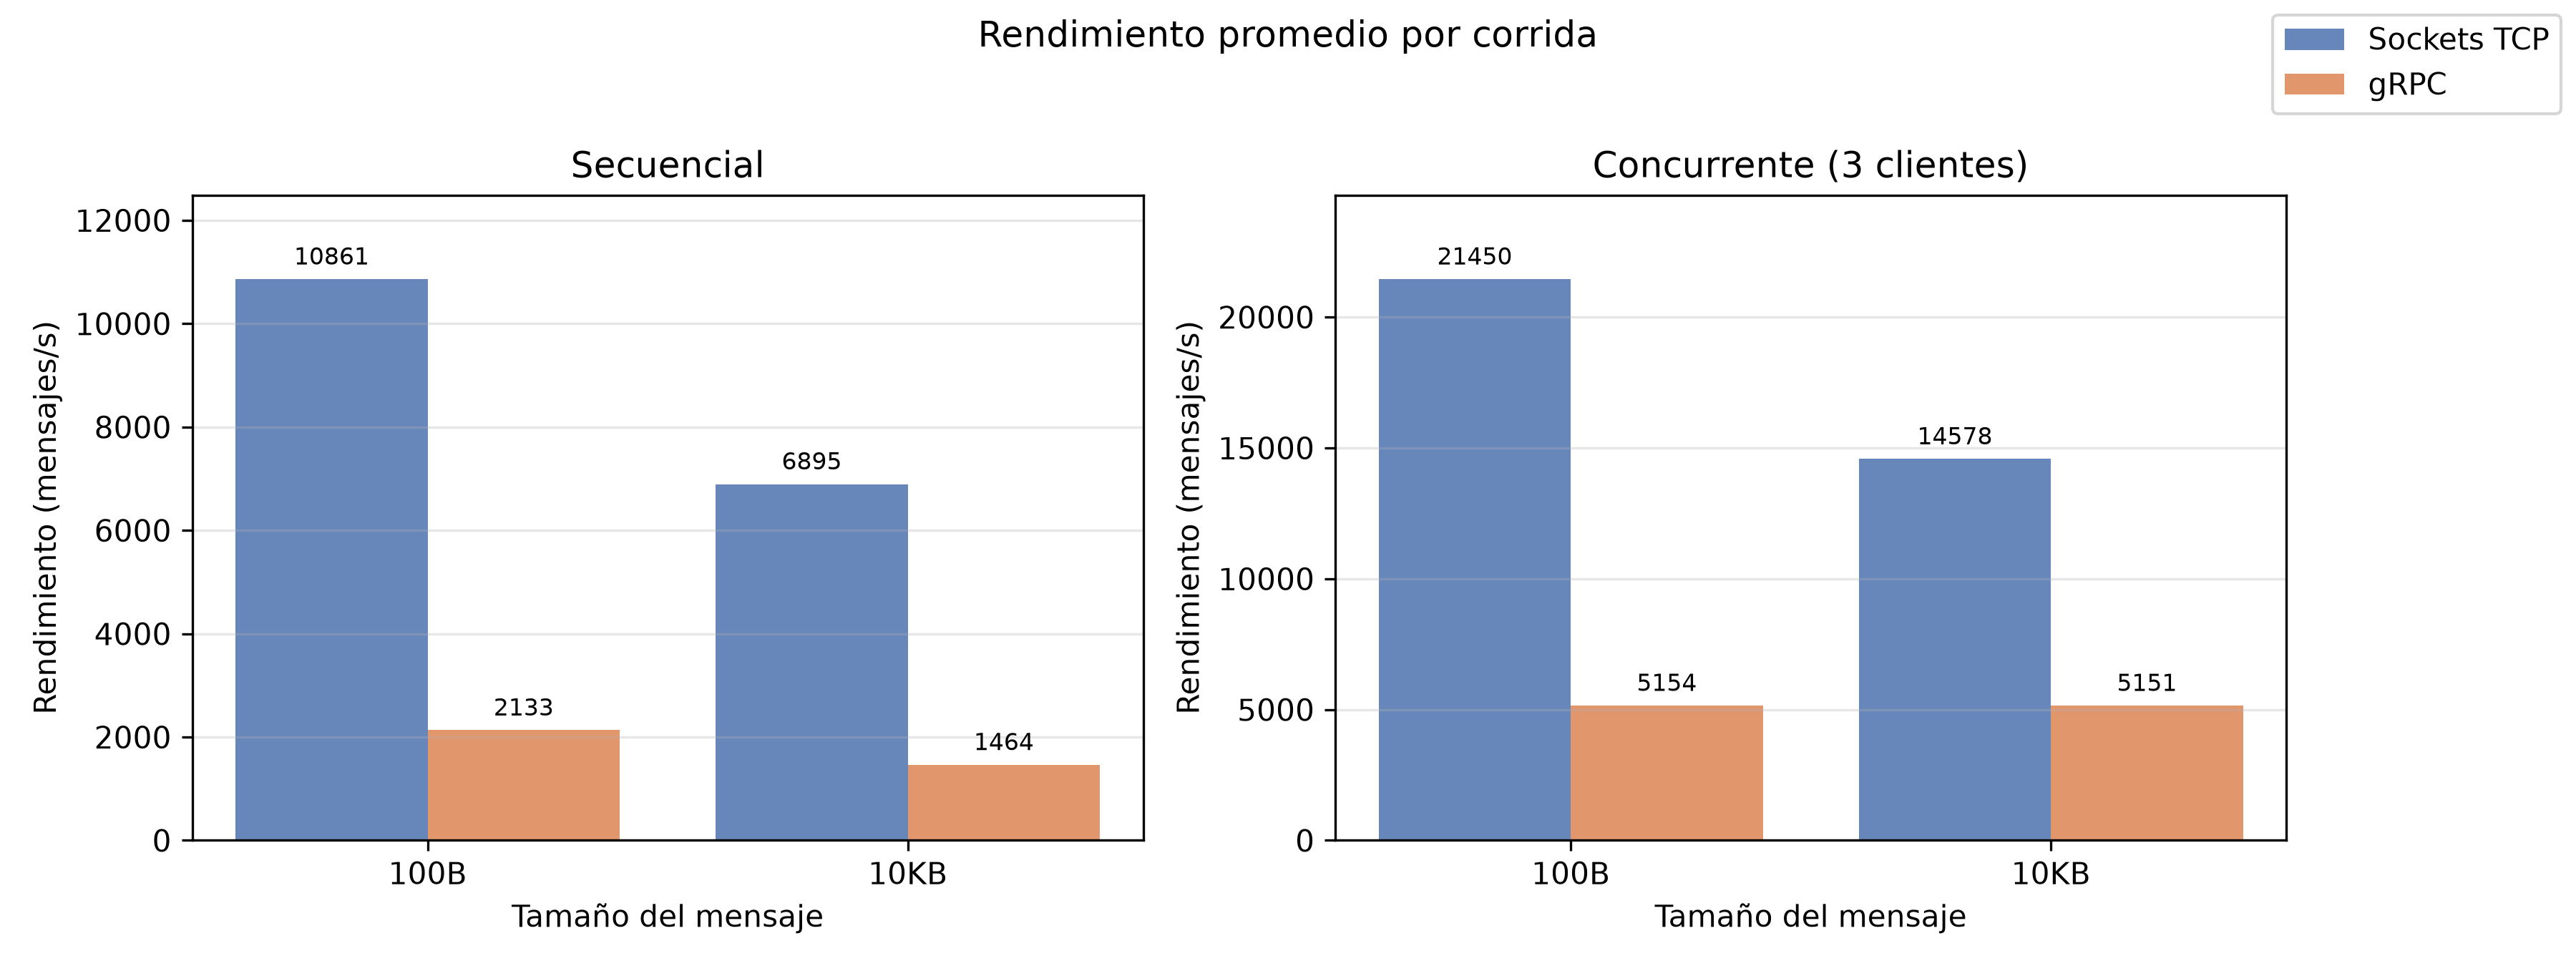
\includegraphics[width=0.96\textwidth]{figures/barras_rendimiento.png}
\caption{Rendimiento promedio por corrida (mensajes/segundo) en modo secuencial y con tres clientes concurrentes (300\,DPI).}
\label{fig:barras_rendimiento}
\end{figure}

El diagrama de cajas (Figura~\ref{fig:boxplot_latencias}) evidencia que Sockets TCP concentra sus observaciones en rangos intercuartílicos estrechos y desviaciones estándar bajas (0,0221--0,0600\,ms). En gRPC la dispersión es mayor (0,0928--0,2951\,ms) y aparecen valores atípicos hasta aproximadamente 4,2\,ms en el escenario concurrente de 100\,B, atribuibles a la contención del planificador de hilos en Windows y la transición entre Python y el núcleo en C de \texttt{grpcio}. Las Figuras~\ref{fig:barras_latencia_ic95} y~\ref{fig:barras_rendimiento} confirman que los intervalos de confianza al 95\,\% son estrechos ($\pm$0,0019--0,0030\,ms en TCP y $\pm$0,0081--0,0149\,ms en gRPC), descartando que las diferencias observadas respondan a fluctuaciones aleatorias.

\section{Discusión y Análisis Crítico}
\label{sec:discusion}

\subsection{Comparación técnica entre Sockets TCP y gRPC}

\begin{itemize}
  \item \textbf{Latencia y variabilidad:} Sockets TCP logró menor latencia media y menor variabilidad en los cuatro escenarios (entre 2,90$\times$ y 5,27$\times$ más rápido en media, y con una desviación estándar entre 2,79$\times$ y 5,07$\times$ menor). Sobre \texttt{localhost}, la ausencia de entramado HTTP/2, negociación de cabeceras HPACK y encolado en el \emph{pool} de hilos de gRPC reduce el camino crítico de cada mensaje~\cite{liu2022session,ciftci2025review}.
  \item \textbf{Rendimiento y escalamiento:} aunque TCP mantuvo mayor rendimiento absoluto (hasta 21\,449,7\,msg/s frente a 5\,153,6\,msg/s), gRPC mostró mejor estabilidad frente al crecimiento del tamaño de carga útil bajo concurrencia: al multiplicar el mensaje por 102,4 (de 100\,B a 10\,KB), el rendimiento concurrente de TCP cayó un 32,0\,\% (de 21\,449,7 a 14\,577,6\,msg/s), mientras que el de gRPC se mantuvo en 5\,151,1\,msg/s gracias a la eficiencia de la serialización binaria de Protocol Buffers~\cite{jackson2024streaming,mehdi2026crosslanguage}.
  \item \textbf{Facilidad de desarrollo, tipado y manejo de errores:} en Sockets TCP el equipo tuvo que diseñar manualmente el prefijo de longitud de 4 bytes (\texttt{framing.py}), la lectura exacta de fragmentos de 10\,KB (\texttt{recv\_exact}) y la validación de claves JSON en tiempo de ejecución. En gRPC, el contrato \texttt{proto/messaging.proto} impone tipado estático fuerte, genera automáticamente los \emph{stubs} cliente/servidor y proporciona códigos de estado estandarizados (\texttt{UNAVAILABLE}, \texttt{DEADLINE\_EXCEEDED}, \texttt{INVALID\_ARGUMENT}) y \emph{timeouts} nativos por invocación~\cite{niswar2024performance,zhu2025rethinking}.
\end{itemize}

\subsection{Contraste con la hipótesis previa}

La hipótesis formulada antes de medir se cumplió \textbf{de forma parcial}:
\begin{enumerate}
  \item \textbf{Mensajes cortos de 100\,B (confirmada):} tal como se anticipó, Sockets TCP obtuvo menor latencia media (0,0884\,ms frente a 0,4655\,ms; gRPC fue 426,77\,\% más lento) debido al costo fijo del entramado HTTP/2 y las capas de \emph{stubs} sobre interfaz local.
  \item \textbf{Mensajes largos de 10\,KB y concurrencia (confirmada en tendencia, refutada en cruce absoluto):} la diferencia relativa a favor de TCP efectivamente se redujo de forma marcada al pasar a 10\,KB concurrente (de 426,77\,\% a 190,39\,\% en media, y de $-$80,36\,\% a $-$64,66\,\% en rendimiento), y gRPC escaló proporcionalmente mejor al incorporar los tres clientes (3,52$\times$ frente a 2,11$\times$ de TCP). No obstante, gRPC no superó a TCP en latencia ni en P95 porque: (a) el cliente TCP utilizó conexiones persistentes con \texttt{TCP\_NODELAY=1} y un encabezado mínimo de 4 bytes; (b) en CPython, la serialización de una carga plana en JSON (\texttt{json} en C) para 10\,KB sobre \texttt{loopback} continúa siendo más liviana que atravesar las capas de HTTP/2 y el ejecutor de hilos de \texttt{grpcio}; y (c) se activó el \emph{subchannel pool} local en gRPC para igualar el número de conexiones independientes frente a TCP, evitando compartir un único canal multiplexado.
\end{enumerate}

\subsection{Amenazas a la validez}

Cuatro factores pudieron influir en las mediciones y acotan la generalización de los resultados:
\begin{itemize}
  \item \textbf{Despliegue en una sola máquina (\texttt{localhost}):} al eliminar el retardo físico de propagación, el enrutamiento y la pérdida de paquetes, se amplifica el peso relativo del procesamiento en espacio de usuario (donde gRPC paga su pila HTTP/2) respecto a una red LAN o WAN real~\cite{ciftci2025review}.
  \item \textbf{Contención de CPU y ruido del sistema operativo:} los tres servidores y los tres clientes compartieron los mismos 12 hilos lógicos y el planificador de Windows 11 junto con procesos de fondo del sistema, generando los valores atípicos observados en la Figura~\ref{fig:boxplot_latencias}.
  \item \textbf{Naturaleza de la carga útil y cifrado:} los mensajes de 10\,KB contienen una cadena ASCII repetitiva y viajaron sin TLS (\texttt{insecure\_channel} y TCP en claro). Con estructuras anidadas ricas en campos numéricos y cifrado TLS obligatorio en producción, el costo de parsear JSON crecería más rápido que el de Protobuf~\cite{mehdi2026crosslanguage,haindl2024security}.
  \item \textbf{Resolución de la hora física en Windows:} \texttt{datetime.now()} presentó una resolución efectiva cercana a 1\,ms en la captura de eventos; por ello, las latencias se midieron exclusivamente con el reloj monotónico de alta resolución \texttt{time.perf\_counter()} y la verificación de Lamport empareja eventos por \texttt{msg\_id}.
\end{itemize}

\subsection{Respuestas a las preguntas obligatorias de análisis (Anexo 8)}

\subsubsection{1. Influencia del número de nodos en el tiempo de convergencia de los relojes de Lamport}

Los relojes lógicos de Lamport no convergen a una hora física única, sino que propagan el valor lógico máximo mediante el intercambio de mensajes ($L \leftarrow \operatorname{max}(L, t_{\mathrm{rec}}) + 1$). En un sistema de $N$ nodos con diámetro de comunicación $D(G)$, una actualización generada en un nodo requiere al menos $D(G)$ saltos secuenciales para reflejarse en los demás procesos: en una malla completa con difusión basta $D = 1$ salto ($O(N)$ mensajes), en un anillo crece como $D = \lfloor N/2 \rfloor$ y en una cadena como $D = N - 1$.

En los registros reales del experimento con $N = 3$ nodos y 20 intercambios (\texttt{events\_sockets.csv} y \texttt{events\_grpc.csv} en \texttt{/data/}), \texttt{nodo-A} y \texttt{nodo-B} arrancan concurrentemente en $L = 1$ (\texttt{ex-01} y \texttt{ex-02}). Al recibirlos \texttt{nodo-C} avanza a $L = 2$ y $L = 3$; recién tras el envío de vuelta a \texttt{nodo-A} (\texttt{ex-03}, $L = 5$) y el posterior envío hacia \texttt{nodo-B} (\texttt{ex-04}, $L = 7$) la información causal originada en el paso inicial alcanza a los tres procesos (4 intercambios). Asimismo, al finalizar el intercambio \texttt{ex-20}, los relojes quedaron en $L_A = 33$ (12 eventos), $L_B = 37$ (14 eventos) y $L_C = 38$ (14 eventos), con una brecha de 5 unidades para el nodo que no participó en los dos últimos mensajes. En tiempo físico, los 20 intercambios tomaron 201,79\,ms en TCP (abriendo conexión por intercambio) y 14,08\,ms en gRPC (con canales persistentes por par). Si $N$ se incrementa sin comunicación periódica todos-contra-todos, tanto la dispersión lógica entre nodos inactivos como el tiempo físico de propagación crecen proporcionalmente a $D(G) \cdot \mathrm{RTT}_{\mathrm{medio}}$ (en nuestros datos, $\approx$0,088--0,199\,ms por salto en TCP y $\approx$0,466--0,676\,ms en gRPC en red local)~\cite{castello2024inductive,mathur2022treeclock}.

\subsubsection{2. Elección de Sockets TCP frente a gRPC en el PFC desde la perspectiva del teorema CAP}

El proyecto de fin de curso del equipo (\emph{Bolsa de Empleos para Graduados UTEQ --- Sistema Distribuido}) se estructura en cinco microservicios con base de datos independiente por servicio: \texttt{Perfiles}, \texttt{Ofertas y Validación}, \texttt{Postulaciones}, \texttt{Ingesta Externa} y \texttt{Notificaciones}. Al analizar sus enlaces bajo el teorema CAP~\cite{khoshaba2023cap}, donde cualquier red distribuida real está expuesta a particiones ($P$) y obliga a elegir entre consistencia ($C$) y disponibilidad ($A$):
\begin{itemize}
  \item \textbf{Cuándo usar gRPC (rutas críticas \emph{CP}):} en la comunicación interna síncrona entre \texttt{Postulaciones} y \texttt{Perfiles} (mediante \texttt{VerificarElegibilidad} en el servicio \texttt{PerfilService}, puerto \texttt{50051}) y entre \texttt{Ofertas} y \texttt{Perfiles}. En este flujo la consistencia prevalece sobre la disponibilidad: si existe una partición entre ambos microservicios, el sistema no debe admitir una postulación sin comprobar que el graduado cumple los requisitos de la oferta. Aunque gRPC añade $\approx$0,38--0,53\,ms de latencia frente a TCP en laboratorio, ese sobrecosto es despreciable ante una consulta a PostgreSQL (varios milisegundos) y aporta contratos estrictos en \texttt{.proto}, interoperabilidad Java/Python, \emph{deadlines} explícitos y códigos de error tipados que permiten fallar de forma controlada~\cite{niswar2024performance,zhu2025rethinking}.
  \item \textbf{Cuándo usar Sockets TCP:} únicamente si el ecosistema incorporara un agente o servicio legado de muy bajo nivel (por ejemplo, un colector interno de telemetría o integración directa con un sistema universitario antiguo sin soporte HTTP/2 ni Protobuf) donde la prioridad sea minimizar la sobrecarga de protocolo (0,088--0,199\,ms) con un formato compacto fijo.
  \item \textbf{Flujos \emph{AP} (fuera del alcance síncrono):} para \texttt{Notificaciones} e \texttt{Ingesta Externa}, donde se privilegia la disponibilidad con consistencia eventual, ninguno de los dos canales síncronos es óptimo; corresponde comunicación asíncrona mediante colas de mensajes (AMQP) con patrón \emph{outbox} e idempotencia~\cite{mohammad2025resilient}.
\end{itemize}

\subsubsection{3. Comportamiento de los timestamps de Lamport ante el fallo de un nodo}

Si un proceso falla por caída (\emph{crash}) o queda aislado por una partición de red (por ejemplo, \texttt{nodo-B}), el algoritmo de Lamport no impone bloqueo global sobre los nodos restantes. \texttt{nodo-A} y \texttt{nodo-C} continúan incrementando sus contadores con \texttt{tick()} y actualizándolos con $\operatorname{max}(L, t_{\mathrm{rec}}) + 1$ en cada intercambio mutuo, preservando estrictamente la condición de reloj ($a \rightarrow b \Rightarrow L(a) < L(b)$) dentro de la partición activa.

Mientras tanto, el reloj de \texttt{nodo-B} queda congelado (o vuelve a cero al reiniciarse sin almacenamiento persistente). Si posteriormente \texttt{nodo-B} se recupera y emite un mensaje antes de recibir tráfico, su marca lógica será baja ($L = 1$); sin embargo, en el primer mensaje que reciba desde \texttt{nodo-A} o \texttt{nodo-C} (por ejemplo, con $t_{\mathrm{rec}} = 38$), la regla $\operatorname{max}(1, 38) + 1 = 39$ vuelve a situar su reloj por encima del máximo causal conocido en un solo paso. El costo del fallo es la pérdida de trazabilidad de los eventos no confirmados del nodo caído y la necesidad de que los clientes capturen \texttt{ConnectionRefusedError} o \texttt{TimeoutError} (en TCP) y \texttt{UNAVAILABLE} o \texttt{DEADLINE\_EXCEEDED} (en gRPC) para evitar bloqueos indefinidos~\cite{mohammad2025resilient}.

\subsubsection{4. Transparencias ANSA logradas y cómo implementar las faltantes}

\begin{itemize}
  \item \textbf{Transparencias logradas:}
    \begin{enumerate}
      \item \emph{Acceso (alta en gRPC, limitada en TCP):} gRPC oculta la serialización binaria y el transporte HTTP/2 detrás de una llamada a método local (\texttt{stub.EnviarMensaje}), mientras que TCP expone el entramado de 4 bytes y el empaquetado JSON.
      \item \emph{Concurrencia (parcial):} los tres servidores atienden múltiples clientes simultáneos (\emph{threads} por conexión en TCP y \texttt{ThreadPoolExecutor} en gRPC) protegiendo el estado compartido del reloj con \texttt{threading.Lock}, evitando condiciones de carrera en las 6\,000 mediciones concurrentes válidas (3\,000 por mecanismo).
    \end{enumerate}
  \item \textbf{Transparencias faltantes y estrategia de implementación:}
    \begin{enumerate}
      \item \emph{Ubicación:} actualmente las direcciones y puertos (\texttt{127.0.0.1:5000--5002}) están fijos en \texttt{src/common/config.py}. Se lograría con un servicio de descubrimiento dinámico (Consul, etcd o registros DNS SRV en Kubernetes) para resolver nombres lógicos en tiempo de ejecución.
      \item \emph{Migración y reubicación:} mover un nodo a otro host o puerto interrumpe los clientes activos. Requiere un balanceador L4/L7 o \emph{service mesh} (Envoy) junto con reconexión automática y \emph{backoff} exponencial.
      \item \emph{Replicación:} cada nodo corre como instancia única sin copias de respaldo. Se implementaría replicando el estado en grupos con protocolo de consenso (Raft) o réplicas activo-pasivo.
      \item \emph{Fallos:} una caída de servidor aborta la fase actual del cliente. Se incorporaría detección mediante \emph{health checks} (\texttt{grpc.health.v1}), reintentos idempotentes basados en \texttt{msg\_id} y disyuntores (\emph{circuit breakers})~\cite{mohammad2025resilient}.
      \item \emph{Persistencia:} los relojes y registros de eventos residen en memoria volátil hasta su volcado final. Bastaría respaldar el contador y el registro en un \emph{write-ahead log} o base embebida (SQLite) para recuperar el estado tras reinicios.
    \end{enumerate}
\end{itemize}
